\documentclass[12pt]{article}
\usepackage{fullpage}
\usepackage{graphicx, rotating, booktabs} 
\usepackage{times} 
\usepackage{fbb} 
\usepackage{natbib} 
\usepackage{indentfirst} 
\usepackage{setspace}
\usepackage{grffile} 
\usepackage{hyperref}
\usepackage{tikz-cd}
 \usetikzlibrary{cd}
\usepackage[export]{adjustbox}
\usepackage[most]{tcolorbox}
\usepackage{verbatimbox}
\usepackage{lscape}
\usepackage{afterpage}
\usepackage{amsmath}
\usepackage[labelfont={bf},textfont=it,labelsep=period]{caption}
 \usepackage{multirow} 
\setcitestyle{aysep{}}
\usepackage{dcolumn}

\hypersetup{
  colorlinks = true,
  urlcolor = blue,
  linkcolor = black,
  citecolor = black,
  pdfauthor = {Joshua Alley},
  pdfkeywords = {},
  pdftitle = {},
  pdfsubject = {},
  pdfpagemode = UseNone,
%  pdffitwindow = true
%  pdfcenterwindow = true
}



\singlespace
%\title{\textbf{Elections, Arms Deals and Autocratic Allies}}
\title{\textbf{Arms and Electoral Influence: How Arms Deals with Autocratic Allies Encourage Defense Contracting Cycles}}
\author{Joshua Alley \\
Assistant Professor \\
University College Dublin\thanks{Thanks to Brian Blankenship, Jonathan Caverley, Jonathan Chu, Ben Fordham, Erik Lin-Greenberg, Zachary Markovitch, Pieter Wezeman as well as participants in the Boston University Political Economy of Security Online Workshop Series and 2022 Meeting of the International Studies Association for helpful comments.} \\
joshua.alley@ucd.edu
}

 
\date{\today}

\bibliographystyle{apsr}

\usepackage{sectsty}
\sectionfont{\Large}
\subsectionfont{\noindent\large\textit}
\subsubsectionfont{\normalsize}

\makeatletter
\renewcommand\tiny{\@setfontsize\tiny{9}{10}}
\makeatother


\begin{document}

\maketitle 

\begin{abstract} 
Arms deals with U.S. allies, especially autocratic partners, facilitate electoral cycles of defense contracting in the United States. 
U.S. leaders make arms deals so they can use defense contracting to stimulate the economy in key electoral areas.
%Presidents and senators use defense contract for economic stimulus because they have more control over this instrument than aggregate economic policy.
Autocratic alliance prot{\'e}g{\'e}s have more need and political flexibility to strike arms deals near elections. 
I examine these claims by analyzing the electoral determinants of defense contracting and arms export deals by the United States. 
First, I  detail electoral cycles in arms deals between the United States and its allies. 
I then use prime contracting data to show correlations between electoral competition and state-level contract awards. 
Third, I employ Bayesian models to link defense contract awards around elections directly to arms deals and then examine sectoral differences in weapons deals and contracting.
The results suggest that.... 
\end{abstract} 


\newpage 
\doublespace 


\section{Introduction}



% US-Brazil 1972
In 1972, the Nixon administration struck ten different deals to transfer or sell arms to Brazil.
Over the next four years, Brazil's military dictatorship received 500 M-113 armoured personnel carriers, five destroyers, seven submarines, and eight S-2E Tracker anti-submarine warfare aircraft.
These deals came while Nixon sought reelection and subsequent deliveries continued after his 1974 resignation. 


% Obama 2012
Similar events took place in 2012, when Saudi Arabia ordered a large arms package from the Obama administration.\footnote{Obama first announced the deal in 2010.} 
Twelve deals included 400 Harpoon anti-ship missiles, 12 Apache attack helicopters for the Saudi National Guard, and 63 K-6 120mm mortars, along with parts for F-15 aircraft, guided bombs, and other helicopters. 
Deliveries of these systems and other weapons spanned the next eight years, including the 2015 Saudi intervention in the Yemeni civil war.\footnote{All deal information from \citep{Sipri2022}.}


% example- PBC consequences vary w/ security coop
These examples reflect a more general pattern, where electoral competition in the United States encourages arms deals with allies, particularly autocracies.
Arms deals help leaders use defense contracting to improve economic conditions in areas with high electoral competition \citep{Tufte1978, Mintz1988, Mayer1995, DerouenHeo2000, Becker2021}. 
Electoral cycles in arms deals boost political budget cycles in defense contracting.


% arms exports logic
Alliance prot{\'e}g{\'e}s provide a key market for arms sales in part because leaders can easily justify transfers. 
Allies receive more arms from their patrons near elections because they control import decisions and receive security benefits. 
Autocratic allies are especially important because they receive more arms than other partners \citep{McManusYarhi-Milo2017} and autocrats have few constraints on accommodating electoral cycles.
%These arms export cycles reinforce cooperative relationships between U.S. leaders and alliance prot{\'e}g{\'e}s. 


% Findings
I scrutinize my argument connecting defense contracting, autocratic allies and arms export cycles in three steps. 
First, I examine how electoral competition drives contract awards in an analysis from 2000 to 2020.
I then analyze U.S. arms deals from 1950 to 2019, and show that arms deals with autocratic allies increase as presidential elections approach, while dealmaking with democratic allies remains consistent. 
Finally, I connect contracting and arms deals with multilevel statistical model, and link deals and arms contracts within specific sectors.


% focus on the U.S.
The argument and analysis focus on the United States because it is a leading arms exporter, maintains expansive alliance ties, and has prior evidence of defense contracting cycles. 
While other countries with smaller economies and defense industries might behave in similar ways, deals and contracting cycles will be weaker or absent.
Regardless the pivotal economic and security roles of the United States make understanding the economic and security consequences of U.S. political budget cycles worthwhile.
Furthermore, other states might leverage security cooperation to facilitate different policy cycles. 


% economic and seucrity ties 
The argument and findings address three salient issues in international relations theory and practice. 
First, they reveal that efforts to create political budget cycles have international security consequences. 
Just as domestic political business cycles in large countries like the United States reshape international economic exchanges and have knock-on effects in other countries \citep{Kayser2006, Kayser2009}, electoral competition alters security cooperation. 


% coercion
Second, this paper provides new insight into alliance bargaining and statecraft. 
Scholars often address coercion and divergent preferences in alliances \citep[pg. 122]{Oatley2015}, \citep{Beckeretal2023}. 
But as \citet{Baldwin2020} notes, statecraft includes positive inducements and negative sanctions. 
This paper highlights positive statecraft by alliance prot{\'e}g{\'e}s, who use arms deals to cooperate with a key patron.
As a result, it connects with prior work on issue linkage in alliance management, including studies of alliance formation \citep{Poast2012} and credibility \citep{Davis2008, Poast2013}.
In this instance, patron leader and prot{\'e}g{\'e} security incentives align well.


Finally, my findings complement prior findings that foreign states' economic policies impact electoral competition. 
\citet{KimMargalit2021} find that Chinese tariffs reduced Republican vote share in the 2018 midterm elections by targeting industries in competitive districts.
In the same way, \citet{ChyzhUrbatsch2021} find that Chinese soy tariffs hurt Republican congressional candidates in soy-producing areas. 
My argument inverts these findings by examining how security cooperation facilitates electoral budget cycles and helps incumbents. 
As a result, small states exert big indirect influence on alliance patrons \citep{Keohane1971}.


% policy (THINK HARD ABOUT CUTTING)
%Allied accommodation of political budget cycles by taking arms exports has important implications for alliance durability. 
%Leaders who anticipate allied orders to stimulate defense contracting cycles will be more likely to demonstrate and uphold alliance commitment. 
%Arms deal cycles are a potential component of larger bargains between alliance patrons and their prot{\'e}g{\'e}s. 


% need an outline 
The paper proceeds as follows. 
To start, I outline an argument detailing the international consequences of political business cycles in the United States, the role of defense contracting in those cycles, and the consequences for arms deals. 
I then test the process in three steps. 
First, I establish the political business cycle roots of arms exports with evidence of defense contracting cycles. 
I then demonstrate that arms exports from the United States to allies increase more as presidential elections approach.
Third, I estimate a joint Bayesian model of the process and link contracts with deals for specific weapons.
The last section discusses the results and offers concluding thoughts.


\section{Argument}


This argument explains the interplay between domestic political budget cycles and the international arms trade. 
First, I detail constraints on aggregate budget cycle tools.
I then discuss how presidential control and Congressional influence makes defense contracting an attractive policy tool for manipulating economic conditions around elections. 
Arms deals with allies can accelerate defense contract cycles. 
Among U.S. allies, autocracies with few constraints on their leaders and strong security motivations to curry favor by accepting arms are especially likely to make arms deals around elections.


Electoral considerations impact policy \citep{Nordhaus1975}.\footnote{See \citet{Dubois2016} for a review of the vast political budget cycle literature.} 
Leaders create political budget cycles by using fiscal and monetary policy to increase economic growth near elections and retain power for themselves or their party \citep{Tufte1978, Rogoff1987}. 
The composition and magnitude of these cycles varies. 
For example, strong central bank interdependence and fixed exchange rates make fiscal cycles more likely \citep{ClarkHallerberg2000}. 
%Even some independent central banks exhibit modest cyclical behavior, however \citep[pg. 247]{Dubois2016}


How leaders bolster economic growth vary with national political institutions. 
Federal Reserve independence limits political influence on monetary policy in the United States, for instance.\footnote{Both Lyndon Johnson and Donald Trump had limited ability to browbeat Federal Reserve Chairs into changing monetary. 
Johnson sought looser monetary policy before the 1968 presidential election, but Fed Chair William McChesney Martin continued to tighten policy.
Trump's tweeted demands for looser monetary policy to increase growth before the 2020 election similarly had little impact on Jerome Powell.}
Recent scholarship also highlights specific policy cycles because leaders struggle to manipulate aggregate economic instruments where they have more direct influence. 
In fiscal policy, aggregate budgets often give leaders limited spending discretion.


Limited flexibility with aggregate instruments encourages democratic leaders to use targeted policies that maximize the electoral impact of their limited discretion.
Some spending shifts can be more narrowly tailored \citep[pg. 248]{Dubois2016}.
Leaders also employ other policies such as trade disputes \citep{Conconietal2017}, labor agreements \citep{Ahlquist2010} and land reform \citep{Philips2020} to win support in key constituencies.


% Defense spending/contracts as flexible instrument
Scholars have long speculated that defense spending is a useful instrument for budget cycles (e.g. \cite{Tufte1978, Mintz1988}).
Executive leaders often have more discretion in defense resource allocation, and defense spending has economic ramifications.
\citet{WhittenWilliams2011} note that defense spending can serve social welfare goals and \citet{Becker2021} finds that unemployment in NATO members encourages leaders to shift spending from equipment to personnel.


% in US context, contracts
Recent studies in the United States argue that defense budgets are poor political cycle tools, however, as Congress makes allocations two years ahead.
This shifted attention towards defense contracting, as leaders control contract timing and disbursement \citep{Mayer1995, DerouenHeo2000}.
Giving contracts also allows leaders to target key constituencies in response to unemployment and approval shifts by claiming credit for awards \citep{DerouenHeo2000}. 


% demand
Contracting is still somewhat constrained by the Congressional budget process, however. 
Leaders can allocate contracts within the budget, but further increases are harder to implement. 
Moreover, should leaders want to increase spending, even the U.S. military may lack absorption capacity to incorporate defense contracting outputs.
Put differently, increased spending from electoral cycles in defense contracting does not respond to military demand, so it requires other buyers. 


When leaders seek to increase spending on defense contracting, foreign markets provide alternative outlets.
When contracting cycles produce new goods, U.S. leaders can also sell or transfer old equipment to partners to make room.
Efforts to use defense contracting for political gains thus has international consequences.\footnote{% Political Business cyles
Other work examines the international economic consequences of budget cycles.
Fiscal and monetary policy shifts impact currency prices and economic growth, which then alters trade and financial ties. 
Economic interdependence leads to correlated economic growth across countries \citep{ArtisZhang1999, Kayser2006} and increases the global economic influence of large economies. 
\citet{Ito1991} finds that U.S. elections increase economic growth in Japan, while \citet{ThompsonZuk1983} uncover some evidence of similar cycles in advanced industrial economies.
\citet{FoersterSchmitz1997} argue that U.S. electoral cycles impact international stock returns.
}


% timeline and intermediate goods
These cycles are more likely to be evidence in arms export deals than deliveries. 
Production times for defense goods vary widely. 
Large platforms like ships, tanks and warplanes can take years to assemble, while munitions and smaller platforms take less time. 
Still, if foreign states place orders for these platforms near elections, contracts can go out quickly.


% additional production and foreign markets
%When defense production and planning diverge, foreign markets provide alternative takers for excess arms production from defense contracting cycles. 
Not all countries are equally likely to make arms deals with the United States near elections, however. 
U.S. allies are more likely to take arms exports than other states. 
Security partners are a pivotal outlet because alliances facilitate security, economic and political cooperation.
The United States often transfers or sells arms to alliance prot{\'e}g{\'e} s, and these states have means and motivation to accommodate electoral cycles. 



\subsection{Alliances and U.S. Arms Exports}


% basic asymm alliance framework
In asymmetric alliances between large and small states, a larger patron protects a smaller prot{\'e}g{\'e}  in exchange for foreign policy concessions \citep{Morrow1991}.
A credible promise of military support increases the patron's foreign policy influence. 
Small alliance members garner protection from external threats and sacrifice some foreign policy autonomy.



Electoral cycles in arms exports to allies benefit U.S. leaders.
Presidents gain capacity to manipulate economic conditions with defense contracting and signal support for U.S. alliance prot{\'e}g{\'e} s by sending arms.
Defense contracting cycles increase prosperity in key electoral areas, which increases a leader's odds of winning office for themselves or their party.\footnote{\citet{Yarhi-Miloetal2016} argue that arms transfers sometimes substitute for formal alliances so patrons can provide security while managing entrapment risk.}


% potential markets: allies
% take new or used stuff to make room
U.S. allies are an obvious market for outputs from political cycles in defense contracting, in part because arms transfer channels are well-established, so negotiations have fewer start-up costs and can build on prior deals.\footnote{I focus here on formal and informal allies, because formal treaties like NATO are not the only U.S. security commitments. Taiwan, Israel and Saudi Arabia have informal security guarantees, and often receive U.S. arms.}
\citet{Thurneretal2019} find that while the relative importance of security and economic factors fluctuates, alliances consistently increase arms transfers.
Common security interests and economic integration of defense industries create economic and security ties that encourage arms trade \citep{Bitzinger1994}. 
Defense industry integration generates trade in intermediate defense goods \citep{Brooks2005}. 
As a result, U.S. allies use weapons, systems and doctrines that facilitate deals for additional arms. 


% less export cycles to non-allies
% each evidence sentence could be its own paragraph 
Allies are more likely than other states to receive arms around elections, and autocratic partners are especially likely to make arms deals. 
The security externalities of arms transfers constrain electoral cycles in arms exports to non-allies. 
U.S. elites will be less willing to increase the capability of states with fewer common interests, even if it facilitates electoral cycles.
Competing elites are also more likely to object to arms deals with non-allies, with electoral costs if they go public with those criticisms \citep{Saunders2022}.
Furthermore, arms transfers outside of alliances could face greater opposition scrutiny near elections, leading presidents to forestall criticism by forgoing contentious transfers.
Limited defense industry cooperation also constrains exports outside alliances to finished goods, while allies with defense industrial ties can receive intermediate goods.



% positive statecraft tie-in from Baldwin 
Allied leaders also benefit from arms exports around elections, because arms exports curry favor with an alliance patron, bolster military capabilities and deepen perceived commitment.
Helping patron leaders with arms deals will dispose them more favorably towards an ally. 
Allies increase their military capabilities with new arms as well, which can make their fighting forces more effective. 
Finally, because arms exports are a costly signal \citep{McManusYarhi-Milo2017}, allies gain confidence in their patron's commitment. 


Arms deals are therefore positive economic and security statecraft by allies. 
Purchases and transfers are a common way that states bolster their political influence \citep[pg. 42-3]{Baldwin2020}.
In alliance politics, \citet[pg. 184-5]{IkenberryGrieco2003} note that states often use direct transfers to attract and sustain security commitments.  


% Sales and transfers- who pays for what
Moreover, prot{\'e}g{\'e} s do not always pay for U.S. arms.
The United States often subsidizes or gifts arms transfers through foreign military sales programs. 
While these still count as arms exports, they impose few immediate costs on recipients.
Alliances make such subsidized transfers to allies easier for presidents to justify to other elites, as they promote common security interests. 


\subsection{Arms Deals for Autocratic Allies}


While all allies might benefit from U.S. arms exports, autocratic allied leaders are more likely to make arms deals near elections. 
Autocracies have fewer domestic political constraints, which frees them to respond to U.S. defense contracting cycles.
They also have stronger security motivations to use arms deals to improve relations with the United States, because arms transfers are central to U.S. security guarantees to autocracies.


% to work, allies must have pol  and budget flexibility
Allied leaders must have the political freedom to make arms deals.
Governments are the customer for most arms sales or transfers, so they have more latitude to take arms, which mirrors how political control of firms increases trade policy flexibility \citep{Davisetal2019}.
At the same time, not every regime is equally free to make arms deals. 


% constraints
Autocratic allies of the United States have greater political flexibility to make arms deals around elections. 
Unlike democratic leaders who might face elite scrutiny of decisions to take additional U.S. arms, for example through legislative opposition, autocrats can strike a deal. 
Even if other domestic actors in an autocracy are opposed to additional outlays on U.S. arms, they have few ways to constrain the leader.\footnote{This changes when opponents of U.S. arms deals are part of the autocrats power base.}


% offstage signaling and need
Ability and motivation are present when autocrats take U.S. arms. 
The United States prefers ``offstage'' signals of support for autocrats, rather than public demonstrations of commitment \citep{McManusYarhi-Milo2017}.
Arms transfers are a pivotal signal of support in these relationships, and sometimes substitute entirely for formal security guarantees \citep{Yarhi-Miloetal2016}. 
When arms are the core of how the U.S. provides security, autocrats will be more willing to accept arms both to increase their military capabilities and signal continued alignment with the United States.


% further need- no ideological affinity
Autocrats also have fewer other tools to curry favor with U.S. leaders.
Formal alliances might promote democratization \citep{GiblerWolford2006, Warren2016}.
The U.S. public is less likely to approve of alliances with an autocrat \citep{Alley2022}, so autocrats have less capacity to pursue deeper ties in other areas. 
The net result is that arms deals are central to U.S. ties with autocratic security partners, so autocrats are more likely to make arms deals near elections. 


% deliberate or not?- key for statecraft argument. 
This argument is agnostic about whether allies make a conscious decision to help political budget cycles by taking arms exports.
While they want improve their alliance relationship, U.S. allies need not choose to accommodate electoral cycles in defense contracting.
Allies may receive better terms and more financial support to take additional goods, or take transfers or surplus materiel as a deliberate favor to leaders who have supported their foreign policy interests. 


% objection- more scrutiny of deals around elections
A potential objection to this argument is that striking arms deals with autocrats might be more costly near elections for U.S. leaders, because political opponents could criticize them for it. 
In this telling, elites can make arms deals a more ``front stage'' signal than U.S. leaders would like. 
Even if this, applies, U.S. leaders may still benefit, as arms deals provide concentrated benefits, while opponents are more diffuse. 
Opponents thus face collective action problems that beneficiaries of deals and corresponding contracts do not, and when contracts focus on electorally salient areas, leaders can expect that the benefits outweigh any costs. 



The overall argument process is as follows.
First, U.S. leaders strike arms deals with other states.
This increases contract awards and arms production, amplifying political budget cycles in defense contracting. 
\autoref{fig:arg-process} summarizes this sequence.


\begin{figure}[htpb]
\adjustbox{scale = .95}{
\centering
\begin{tikzcd}[ampersand replacement=\&]
\mbox{Arms Deals} \arrow[r]  \& \mbox{Defense Contracting} \arrow[r] \& \mbox{Arms Production} \arrow[r] \& \mbox{Electoral Budget Cycles}
\end{tikzcd}
}
\caption{Summary of the argument process linking budget cycles in defense contracting to electoral cycles in U.S. arms deals.}
\label{fig:arg-process}
\end{figure}



% Result- increased exports, tied to electoral cycles
The result of this process is more arms deals as elections approach, especially with autocratic alliance prot{\'e}g{\'e}s.
Arms exports in turn are rooted in electoral cycles of defense contracting.



\subsection{Implications}



The argument generates several testable implications, albeit within the scope of U.S. alliances. 
These twin cycles of arms deals and defense contracting are the result of a large defense industry and many security commitments.
Fixed election scheduling further reduces endogeneity between policy decisions and election timing. 
Other states may have weaker cycles, or electoral cycles in different goods.


The first hypothesis predicts corresponding cycles in arms exports, especially to autocratic allies.
Proximity to presidential elections will increase arms transfers from the United States to autocratic allied states. 


\begin{quote}
\textsc{Arms Deals Hypothesis: As time to a presidential election decreases, U.S. arms deals with autocratic allies will increase.}
\end{quote}


The second prediction tests the expected relationship between defense contracts and arms exports. 
I expect electoral cycles in defense contacting, and a positive correlation between these cycles and U.S. arms exports.


\begin{quote}
\textsc{Defense Contracts Hypothesis: As electoral competition in a state increases, prime defense contract awards increase.}
\end{quote}



% What's next
In the following, I examine each of these hypotheses. 
In the first analysis, I use a series of descriptive data and single-outcome statistical models to illustrate each step in the process.
This starts with descriptive data on defense contracting from 2000 to 2020, then shows how arms exports to allies track U.S. electoral cycles, and ends with a model of electoral cycles in U.S. trade. 
After that, I unify the different outcomes in Bayesian model that captures the process where contract allocations to electorally important states filter up into arms exports, ultimately driving increased exports.



\section{Arms Transfers and Presidential Elections}


The arms deals hypothesis predicts electoral cycles in U.S. arms deals with autocratic allies.
To test this hypothesis, I model U.S. arms deals from 1951 to 2014 using deals data from the SIPRI Arms Transfer Database \citep{SIPRI2021}.
The outcome in this panel dataset of all states outside the United States is the annual count of deals, based on SIPRI's trade register. 
This section presents count data regression estimates of annual arms deals. 


% Why focus on deals
I analyze arms deals rather than observed arms transfers for three reasons.
First, elites can announce arms deals and related contracts immediately. 
Secondly, deliveries can take years after a deal is announced, even for second-hand or aid transfers of existing equipment. 
Finally, deliveries often space out the total value of a shipment over several years, especially for deals with many weapons or larger platforms. 


% key independent variables- ally/partner, 
The argument suggests that three variables driving U.S. arms deals. 
The first is electoral competition, which I measure with an indicator of the number of years to a presidential election. 
The second key factor is whether a country is a U.S. ally. 
I measure alliance status with a binary indicator of whether a country is a formal U.S. treaty ally using data from the ATOP project \citep{Leedsetal2002}, as well as one of three states that have not always had a formal treaty commitment but are widely seen as U.S. allies with implicit security guarantees; Israel, Taiwan and Saudi Arabia. 
I include informal allies because in some of these cases arms substitute for a formal alliance, but the United States is still attempting to ensure partner security \citep{Yarhi-Miloetal2016}. 
Finally, I measure country democracy using the VDem project's polyarchy measure \citep{Coppedgeetal2008}. 
I interact all three of these variables to predict arms deals. 


% models
To estimate how alliances, democracy and election timing shape arms deals, I use a Poisson model.
This fits the annual count of arms deals well.
To preserve compatibility with a later joint model, I use Bayesian estimation with the brms package for \textsf{R} \citep{Buerkner2017}. 
I show in the appendix that OTHER MODELS HERE give similar inferences. 


Along with the three key independent variables, I adjust for other factors that are correlated with arms deals, alliances, and democracy. 
The first control variable is a binary indicator of Cold War years, as more U.S. allies were autocratic during this period. 
I also adjust for EU membership as a potential constraint on some states. 
Further country-level controls include logged GDP, population, and distance the from United States, as well as a binary indicator of common language. 
Finally, I adjust for presidential partisanship with a dummy indicator of years with a Republican president.  



\subsection{Results}


Because interpreting coefficients in triple interactions is challenging, I summarize the interaction of alliances democracy and presidential election proximity in \autoref{fig:us-arms-plots}.\footnote{Coefficient estimates are available in the appendix.}
This figure plots predicted arms deals based on proximity to an election and whether a state is a U.S. ally or not. 
Each facet sets recipient democracy at the minimum, first quartile, median, third quartile and maximum.


\begin{figure}[htpb]
	\centering
		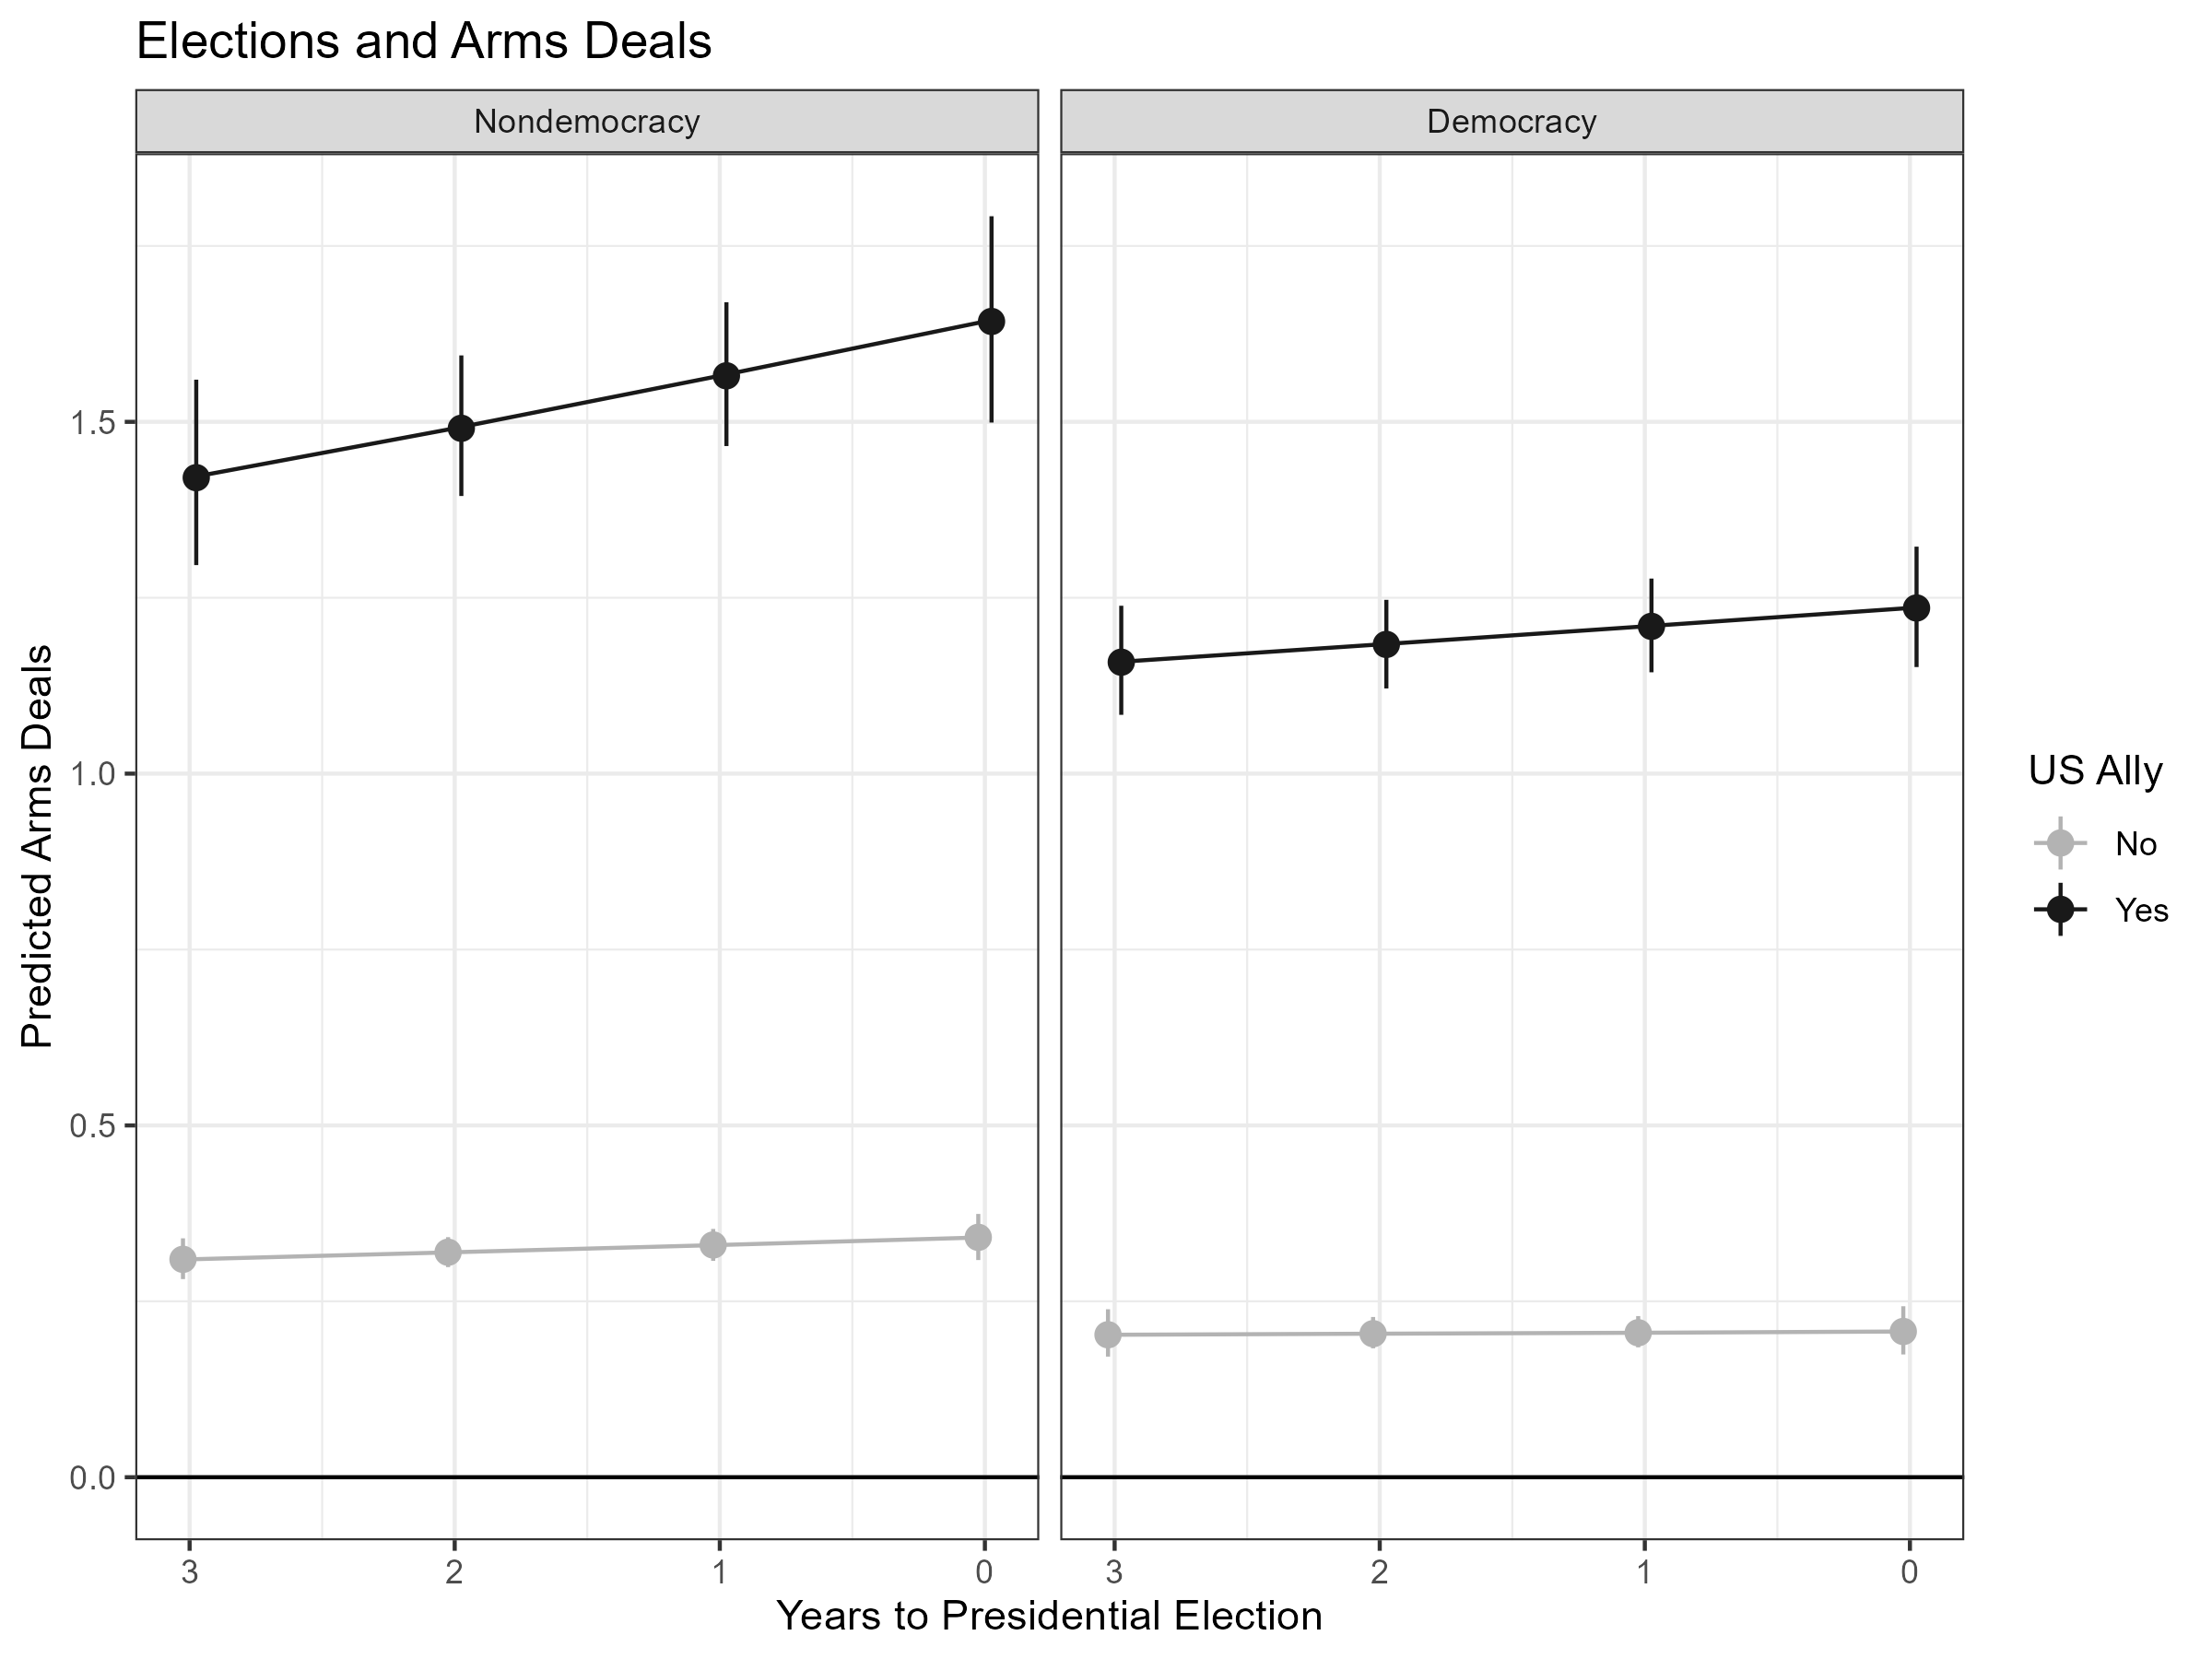
\includegraphics[width=0.95\textwidth]{../figures/us-arms-plots.png}
	\caption{Predicted arms deals between the United States and other states 1950 to 2014 based on presidential election proximity, democracy, and security alliances. Points mark the estimates and error bars summarize the 95\% confidence interval.}
	\label{fig:us-arms-plots}
\end{figure}


There are two key inferences in \autoref{fig:us-arms-plots}.
First, the United States makes more arms deals with allied states than non-allied states, regardless of regime type. 
Predicted deals with non-allied states are low and basically constant across the different levels of democracy. 
The impact of an alliance on arms deals is much greater for autocracies than democracies, however, which is consistent with \citep{McManusYarhi-Milo2017}. 
U.S. allies with minimal polyarchy scores receive one more arms deal a year than states with similar democracy, all else equal. 
Fully democratic U.S. allies receive .4 deals more in expectation. 


The second inference is that electoral cycles in arms deals are present for autocratic allies and absent for democracies.
When allied polyarchy is at the minimum value, predicted arms deals rise from 1.6 to 1.95 throughout the presidential election cycle. 
This cycle diminishes as allied democracy increases, so fully democratic partners see no change in arms deals as elections approach.  


The overall results thus suggest the arms deals hypothesis. 
As presidential elections approach, arms deals rise, but only with autocratic allies. 
Arms deals with democratic allies are unchanged by electoral competition.


These arms deals with autocratic allies near elections are connected to electoral cycles in defense contracting. 
If there are no cycles in defense contract awards, then arms deals have less tangible consequences. 
The next analysis checks for electoral cycles in defense contracting awards. 



\section{Defense Contracting Cycles}


To show electoral cycles in defense contracting, I draw on Department of Defense prime contract award data from the USAspending.gov database.\footnote{Link here: \url{https://www.usaspending.gov/download_center/custom_award_data}.} 
This archive contains data on individual contract awards starting in the 2000 fiscal year, and I collected all Department of Defense contracts from 2000 to 2020.


In addition to aggregating the total federal dollar obligation of all contracts in every year, I differentiate contracts by sector to assess which sectors drive contracting cycles. 
I measure total contracts for aircraft, ships, vehicles, electronics, missiles/space, and weapons/ammunition. 
While large contracts for components of major combat platforms have greater economic heft, full platforms can take years to deliver. 
Missiles, weapons and ammunition may lead to more immediate exports of defense goods, as their production schedules are more flexible.


If defense contracting drives electoral export cycles, we should observe electoral cycles in defense contracting.
\autoref{fig:contract-cycles} shows defense contracting cycles around presidential elections. 
As presidential elections approach, aggregate defense contract awards increase. 
There is a notable spike of \$25-30 billion in the median of overall defense contracts from two years into a presidential term to one year before an election. 
Median defense contracting levels rise further in election years.


\begin{figure}[htpb]
	\centering
		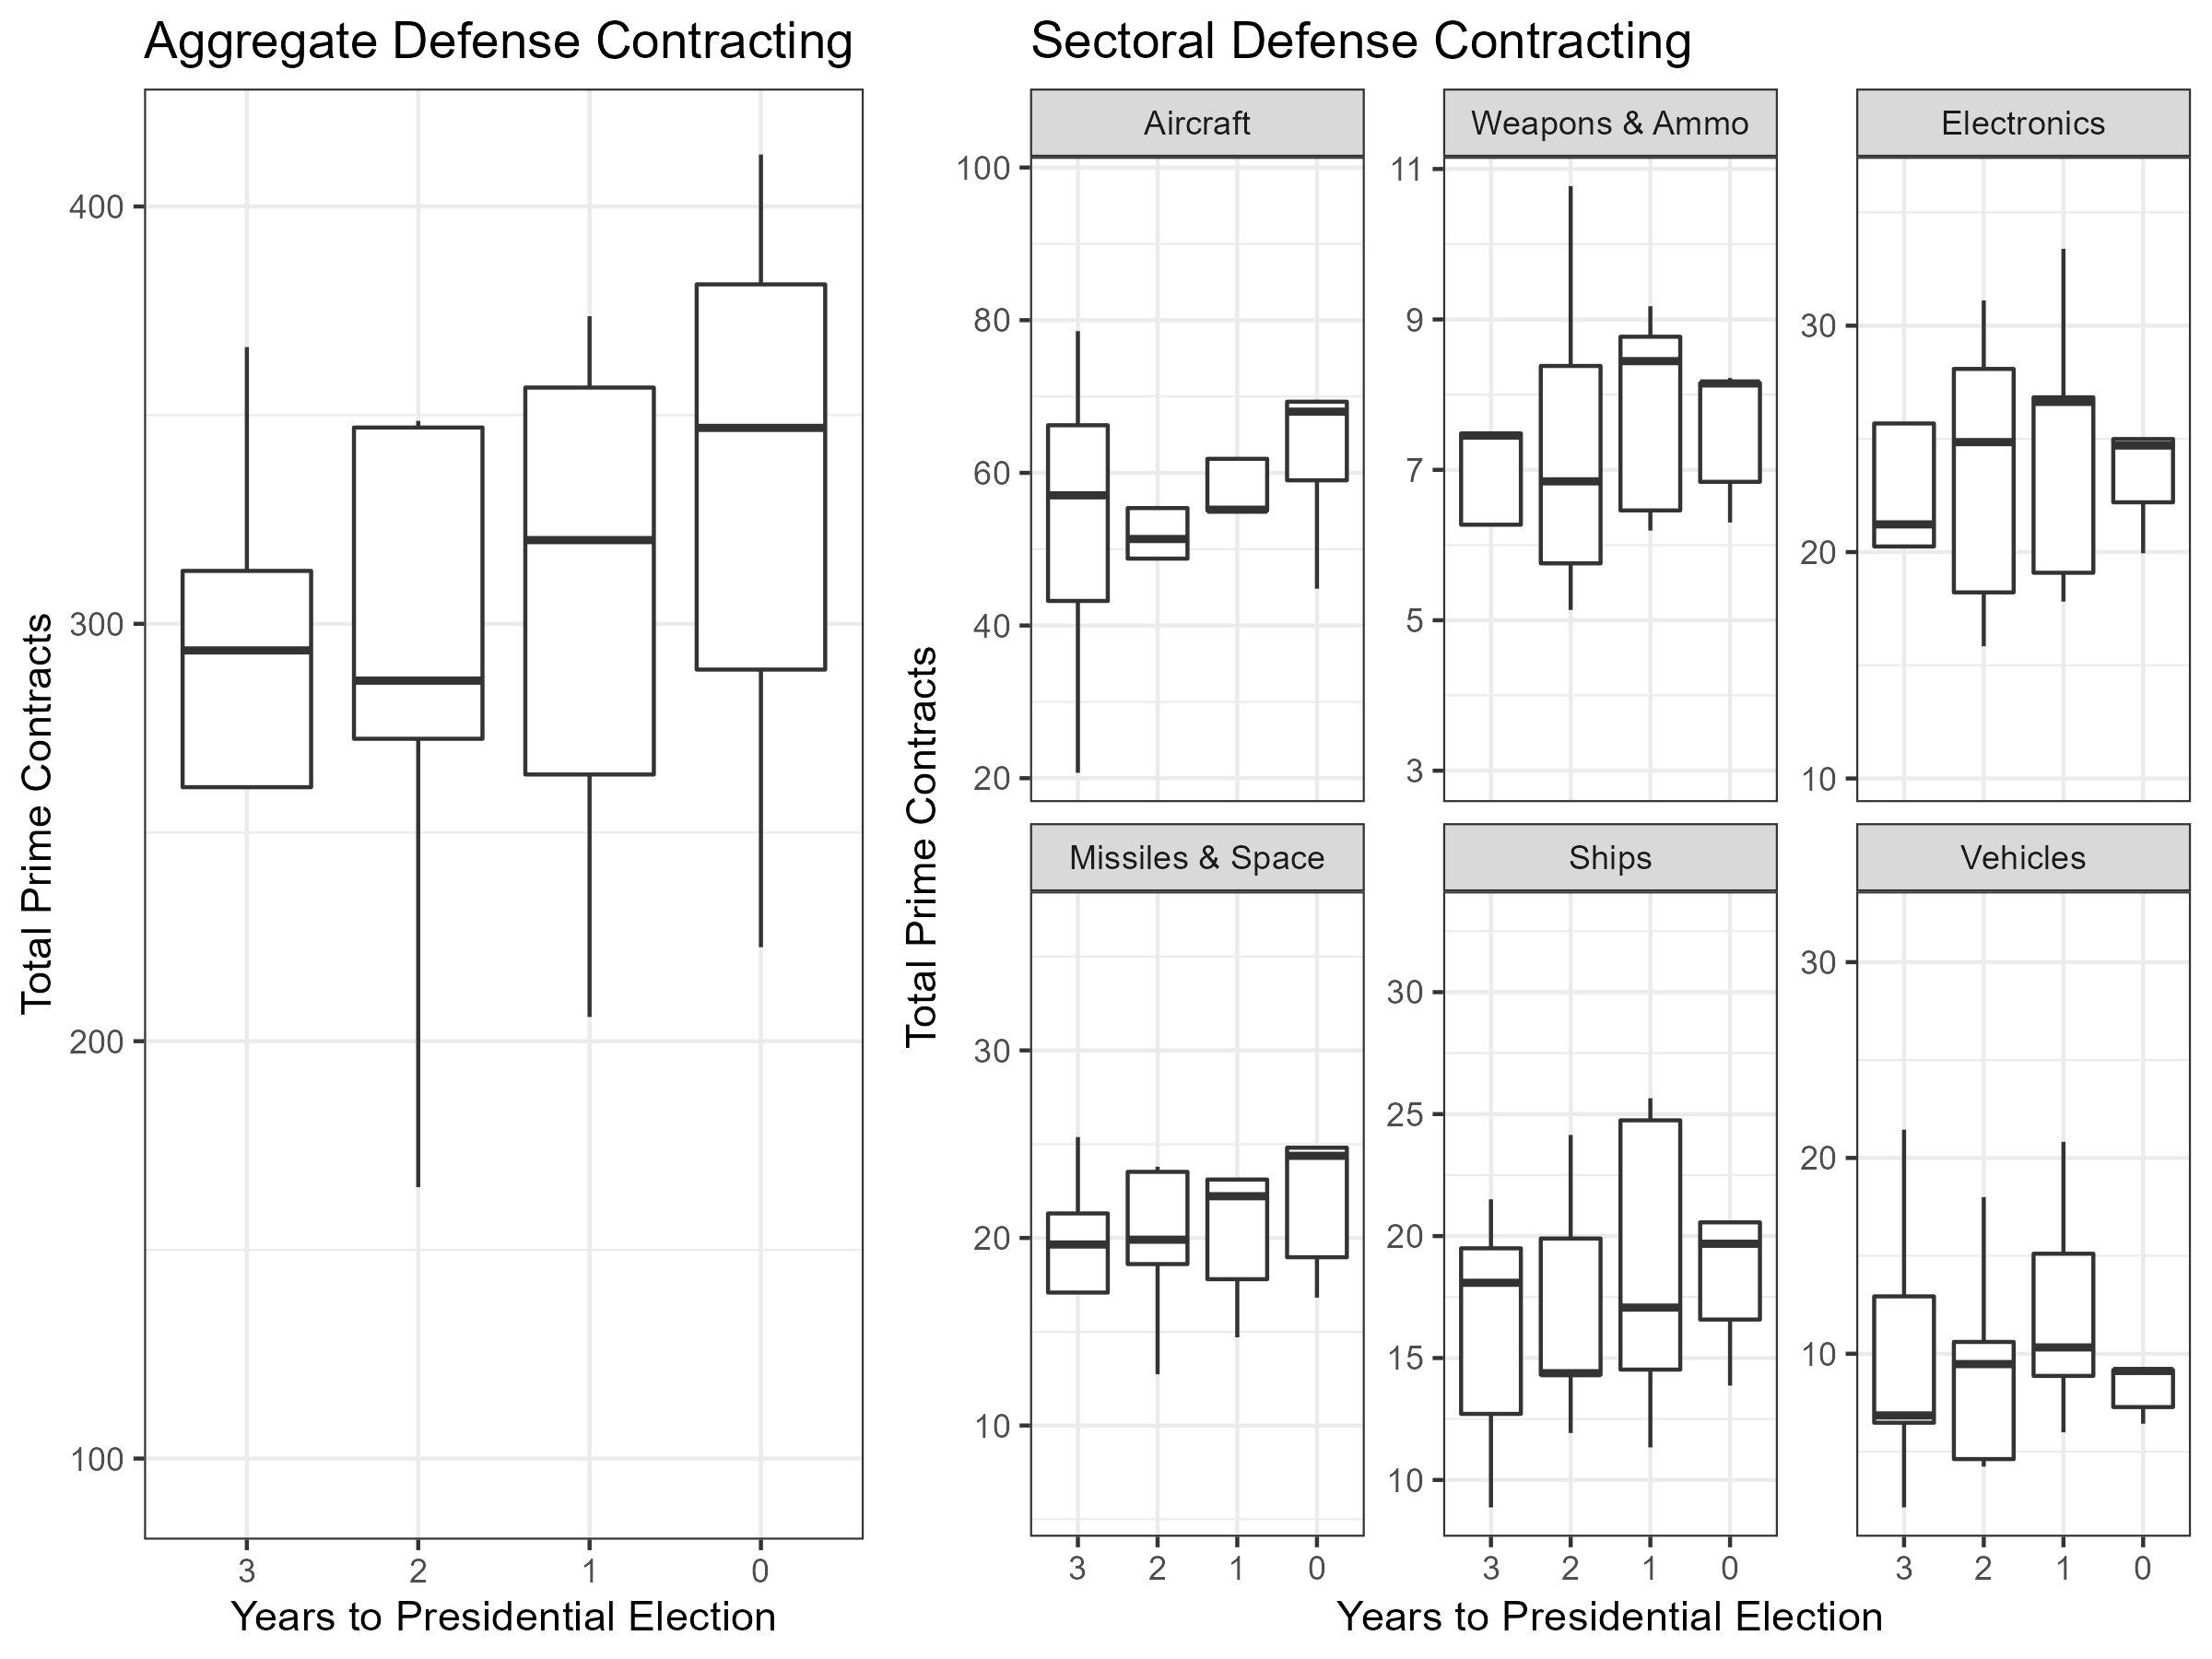
\includegraphics[width=0.95\textwidth]{../figures/contract-cycles.png}
	\caption{Distribution of prime defense contract awards by presidential election proximity, 2000-2020. The dark line in the box plot marks the median value of total contract awards in each year.}
	\label{fig:contract-cycles}
\end{figure}


Particular sectors drive the aggregate increase in defense contracting. 
Aircraft contracts increase dramatically, as do missile and space outlays. 
Naval contacts and prime awards for weapons and ammunition also increase, but retain a high level in the first year of many administrations, which changes those cycles. 
Electronics contracting also rise significantly, and there is a slight increase in vehicle contracting. 
Outside of aircraft, most of the specific platform cycles change the median contract outlay by less than \$10 billion.


Therefore, there is some evidence that defense contracting cycles follow presidential elections.
Along with prior research \citep{DerouenHeo2000}, this suggests that defense contracting is a plausible source of electoral cycles in arms exports from the United States to its allies.
Efforts to manipulate economic conditions through defense contracting have international ramifications. 




\section{A Bayesian Model of Contracts, Arms Exports, and Trade}


The three individual analyses provide initial support for the argument, but they also treat each part of the process in isolation. 
To show the full process, I employ a generative model where each stage of the process informs the next level.
This move 
I employ this approach because standard multiple-equation models in political science cannot easily accommodate divergent levels of analysis.
Flexible structure and Bayesian estimation can capture a wide variety of complex data-generating structures, subject to careful model validation \citep{Betancourt2021}. 





\section{Discussion and Conclusion}


The argument and results suggest that political budget and defense contracting cycles expand international trade, especially arms exports to U.S. allies. 
Economic efforts to bolster presidential electoral prospects have international consequences. 
Additional goods from defense contracting cycles produce arms flows outside the United States.
This bolsters cooperative relations between the United States and its allies.


Allied economic and security statecraft thus helps U.S. leaders win elections. 
While this is not a part of formal alliance bargains, these informal linkages are essential to grand bargains between alliance patrons and prot{\'e}g{\'e}s.
Allies need not undertake these cycles deliberately, but their accepting arms transfers is part of a cooperative bundle of ties regardless.


Allied support for political budget cycles affects democratic alliance credibility and maintenance. 
A stable alliance bargain can develop if leaders anticipate the electoral benefits of defense contracting cycles and arms exports to allies.
When leaders expect that maintaining security commitment will have electoral rewards, they will be more likely to invest in alliances. 


These findings also add an international security component to the political budget cycle literature.
Alliance partnerships can allow leaders to manipulate economic conditions for electoral gain. 
By providing an outlet for defense contracting , allies help leaders contract for new goods with less attention to the absorptive capacity and force planning of the U.S. military.


Finally, the argument and findings add to prior findings that states manipulate international economic and security cooperation to bolster or undermine leaders. 
To give one example, \citet{ChyzhUrbatsch2021} show that Chinese soy tariffs reduced support for Republicans in the 2018 midterm elections. 
Allies have both motive and means to use economic and security cooperation to help leaders. 
Rather than undermine leaders, allied arms import decisions create positive inducements for regular cooperation.


Future research could proceed in several directions. 
First, cycles in other economic outcomes such as foreign direct investment, are an interesting area for study. 
Exploring the role of defense industry integration and intermediate goods in these arms cycles is also critical.
Whether these results generalize to autocratic alliances or other democratic alliance patrons is another worthwhile inquiry. 
Security partners of other alliance patrons may take similar actions in different industries, for instance.


In conclusion, political budget cycles reshape international economic and security cooperation.
Budget cycles increase trade and arms transfers to U.S. allies through economic growth and defense contracting.
Security cooperation can therefore facilitate electoral benefits for leaders. 


\newpage
\singlespace
 
\bibliography{../../MasterBibliography} 


\end{document}